\subsection{Atraminių vektorių klasifikatoriai}

Atraminių vektorių klasifikatoriai (angl. \textit{support vector machines}, SVM) - tai mašininio mokymosi  algoritmas, kuris gali būti taikomas tiek klasifikavime, tiek regresinėje analizėje. Jis priskiriamas prie mokymosi su mokytoju algoritmų \cite{vapnik2000nature}.

Atraminių vektorių klasifikatorių algoritmo idėja yra duomenų vektorių erdvėje surasti hiperplokštumą (sprendimo ribą (angl. \textit{decision boundary})), kurios atstumas nuo skirtingoms klasėms priklausančių objektų būtų didžiausias, galimai pašalinant triukšmą bei išimtis. Kitaip tariant, yra ieškoma hiperplokštuma, kuri geriausiai atskiria objektus priklausančius skirtingoms klasėms. 

Tarkime, kad turime $L$ mokymosi objektų, kurių kiekvienas objektas $x_i$ turi $D$ matų ir priklauso vienai iš dviejų klasių $y_i=-1$ arba $y_i=+1$. Taigi turime mokymosi duomenis, kurių pavidalas yra:
\begin{equation}
 \{x_i, y_i\}, kur\; i=1..L, y_i \in \{-1,1\}, x \in \Re^D
\end{equation}
Tarkime, kad duomenys yra tiesiškai atskiriami. Tai reiškia, kad galima nupiešti tiesę grafe $x_1$ ir $x_2$, kuri atskiria dvi klases, kai $D=2$ ir hiperplokštumą grafuose $x_1, x_2,...x_D$, kai $D > 2$. Hiperplokštuma apibrėžta $w\cdot x + b = 0$, kur $w$ -- hiperplokštumos normalės vektorius, $\frac{b}{||w||}$ -- statmens einančio nuo hiperplokštumos iki koordinačių pradžios taško ilgis.

Atraminiai vektoriai (angl. \textit{support vectors}) yra duomenų objektai esantys arčiausiai atskiriančiosios hiperplokštumos. Atraminių vektorių klasifikatorių algoritmo tikslas yra orientuoti hiperplokštumą tokiu, būdu, kad atstumas tarp jos ir artimiausių objektų iš abiejų klasių \cite{cortes1995support}. Tai pavaizduota ~\ref{fig:support_vector_machines} pav. Taigi, atraminių vektorių klasifikatorių sukūrimas yra parametrų $w$ ir $b$ tenkinančių minėtas sąlygas radimas. Tai galima užrašyti tokia nelygybe:
\begin{equation}
 \label{svm_separable}
 y_i(x_i \cdot w + b) - 1 > 0
\end{equation}
Jei abiejų klasių objektai nėra tiesiškai atskiriami, reikia ,,atpalaiduoti'' (\ref{svm_separable}) salygą:
\begin{equation}
 \label{svm_non_separable}
 y_i(x_i \cdot w + b) - 1 + \xi_i > 0, kur\; \xi_i \geq 0, \;  \forall_i,
\end{equation}
kur $\xi_i$ yra baudos už neteisingai klasei priskirtą objektą dydis.
\begin{figure}
 \centering
 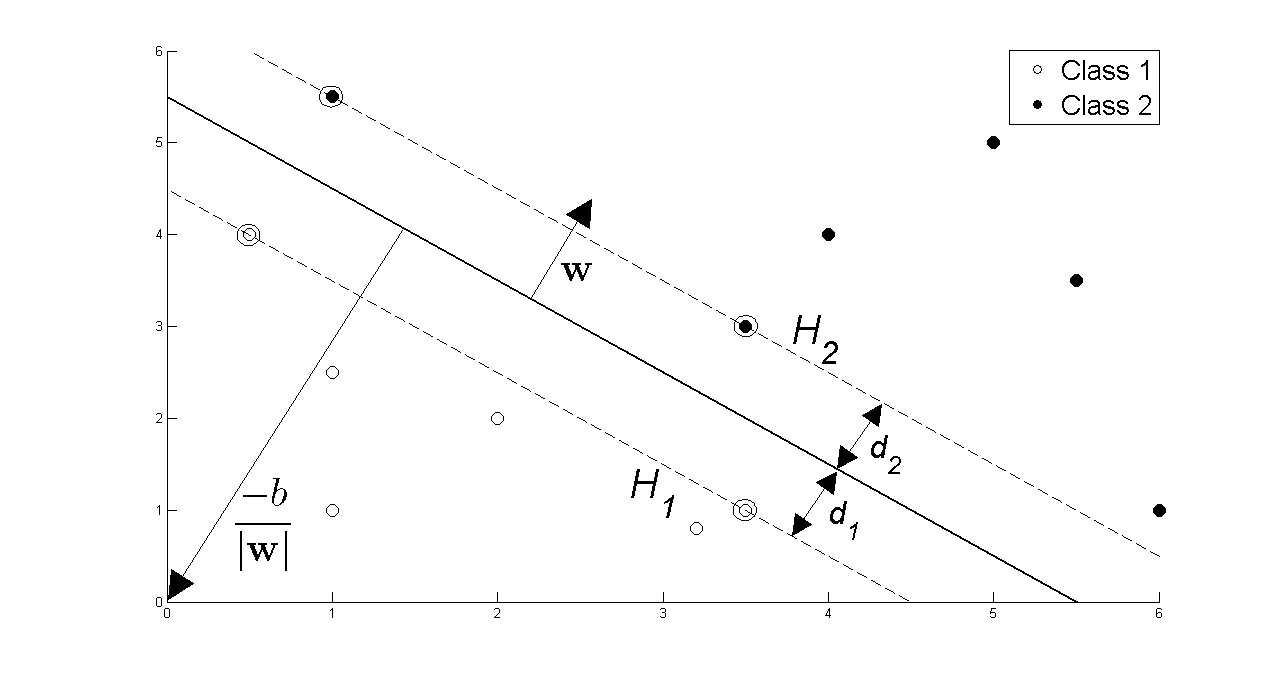
\includegraphics[width=.7\textwidth]{images/support_vector_machines.jpg}
 \caption{Hiperplokštuma nubrėžta per dvi tiesiškai atskiriamas klases.}
 \label{fig:support_vector_machines}
\end{figure}

Atraminių vektorių klasifikatoriai gerai tinka uždaviniams, kai turima labai maža mokymosi duomenų aibė. Biomedicininiai duomenys ir pasižymi tuo, kad mokymosi duomenų aibė yra maža palyginus su turimų matų skaičiumi. Todėl atraminių vektorių klasifikatorių naudojimas dirbui su biomedicininiais duomenimis yra tapęs standartiniu pasirinkimu. 


%% JG: cituoti turi originalų darbą:
%% JG: C. Cortes and V. Vapnik, Support-Vector Networks, Machine Learning, 20(3):273-297, September 1995
%% JG: Vladimir N. Vapnik. The Nature of Statistical Learning Theory. Springer, New York, 1995


%SVM is a type of machine learning algorithm derived from statistical learning
%[theory](http://download.oracle.com/docs/cd/B14117_01/text.101/b10729/classify.htm).

%% JG: nepamiršksio daugiamatiškumo erdvę, o ten juos galima atskirti tiesiškai.